\documentclass[12pt,oneside,paper=a4,headings=small]{scrbook}

\setcounter{secnumdepth}{3}
\setcounter{tocdepth}{3}

% -----------------------------------
% Packages
\usepackage[T1]{fontenc}
\usepackage[ngerman]{babel}
\usepackage{mathptmx}

\usepackage{amsmath}
\usepackage{graphicx}
\usepackage{float}
\usepackage{rotating}
\graphicspath{{bilder/}}
\usepackage{tabularx}
\usepackage{booktabs}
\usepackage{longtable}
\usepackage{array}
\usepackage{listings}
\usepackage{setspace}
\usepackage{lscape}

\newtheorem{mydef}{Key Point}
\newtheorem{bsp}{Example}

% hyperref BEFORE apacite to avoid cite/link breakage
\usepackage[unicode]{hyperref}

% Bibliography package AFTER hyperref
\usepackage{apacite}
\usepackage{tikz}
\usetikzlibrary{arrows.meta, positioning, shapes.geometric}
\emergencystretch=2em
\renewcommand{\arraystretch}{1.2}
% python code formatting
\usepackage{xcolor}

\lstset{
    language=Python,
    basicstyle=\ttfamily\small,
    keywordstyle=\color{blue},
    commentstyle=\color{gray},
    stringstyle=\color{orange},
    numbers=left,
    numberstyle=\tiny,
    breaklines=true,
    frame=single,
    captionpos=b,
    extendedchars=true,
    inputencoding=utf8,
    showstringspaces=false,
    literate=
        {ä}{{\"a}}1 {ö}{{\"o}}1 {ü}{{\"u}}1
        {Ä}{{\"A}}1 {Ö}{{\"O}}1 {Ü}{{\"U}}1
        {ß}{{\ss}}1
}

% -----------------------------------
\begin{document}

\frontmatter
\include{titel/titel}
\newpage

\vspace*{1cm}

\begin{center}
    \textbf{Abstract}
\end{center}

\vspace*{1cm}

\noindent 

Diese Arbeit befasst sich mit der Weiterentwicklung und Evaluation eines am KI-Campus eingesetzten Retrieval-Augmented-Generation-Chatbots im Bildungskontext. Ziel ist es, die bestehende Systemarchitektur und die zugrunde liegende Datenverarbeitung so zu verbessern, dass kontextgestützte Antworten innerhalb eines Lernmanagementsystems qualitativ gesteigert werden.

Grundlage der Weiterentwicklung ist die Analyse von rund 13.000 realen Nutzeranfragen, anhand derer zentrale Nutzungsmuster identifiziert wurden. Daraus werden drei Use Cases abgeleitet: technischer Support, kursbezogene Fachfragen und lernunterstützende Dialoge. Aufbauend auf diesen Erkenntnissen wird die Systemarchitektur gezielt erweitert. Die Implementierung umfasst den Ausbau der Wissensbasis, die Integration multimodaler Inhalte, eine routingbasierte Retrieval-Logik mit Single- und Multi-Hop-Verfahren sowie den Einsatz von Reranking-Mechanismen. Ergänzend werden die Prompt- und Zitierlogik überarbeitet, um Transparenz und Nachvollziehbarkeit der Antworten zu erhöhen.

Die Evaluation der weiterentwickelten Systemversion erfolgt mehrdimensional. Neben automatisierten Qualitätsmetriken werden ein expertenbasierter Blindvergleich im A/B-Design sowie Analysen von Latenzzeiten, Tokenverbrauch und Kosten durchgeführt. Die Ergebnisse zeigen eine verbesserte Kontexttreue, höhere Antwortrelevanz und eine gesteigerte didaktische Qualität. Gleichzeitig wird deutlich, dass die erhöhte Systemkomplexität mit einem höheren Ressourcenverbrauch verbunden ist.

Insgesamt verdeutlicht die Arbeit, dass die Kombination aus technischer Optimierung, empirischer Evaluation und ökonomischer Betrachtung eine fundierte Grundlage für die Weiterentwicklung RAG-basierter Chatbots im Bildungskontext schafft.

\chapter{Abkürzungsverzeichnis}

\begin{tabular}{ll}
AI   & Artificial Intelligence \\
API  & Application Programming Interface \\
ETL  & Extract, Transform, Load \\
LLM  & Large Language Model \\
MCP  & Model Context Protocol \\
RAG  & Retrieval-Augmented Generation \\
RAGAS  & Retrieval-Augmented Generation Assessment System \\
RLHF & Reinforcement Learning from Human Feedback \\
Q\&A & Questions and Answers \\
TAM & Technology Acceptance Model \\
TTFT & Time To First Token \\
UX & User Experience \\
UI & User Interface \\
\end{tabular}


\chapter{Glossar}

\begin{description}
\item[RAG] Kombination aus Retrieval und generativer KI.
\item[TTFT] Time to First Token, Zeit bis zur Ausgabe des ersten Tokens.
\end{description}


\onehalfspacing
\tableofcontents

\addcontentsline{toc}{chapter}{Abbildungsverzeichnis}
\listoffigures

\addcontentsline{toc}{chapter}{Tabellenverzeichnis}
\listoftables

% -----------------------------------
\mainmatter
\chapter{Einleitung}
Die fortschreitende Digitalisierung verändert grundlegende Prozesse der Wissensvermittlung und eröffnet neue Möglichkeiten für individualisierte und adaptive Lernumgebungen. Insbesondere der Einsatz Künstlicher Intelligenz (KI) im Bildungskontext gewinnt zunehmend an Bedeutung, da intelligente Systeme Lernende gezielt unterstützen, Lernprozesse personalisieren und den Zugang zu komplexen Inhalten erleichtern können. Vor diesem Hintergrund rücken dialogische Assistenzsysteme auf Basis grosser Sprachmodelle (Large Language Models, LLMs) in den Fokus der Bildungsforschung und -praxis. Durch ihre Faehigkeit, natürliche Sprache zu verstehen und kontextbezogen zu generieren, ermöglichen sie eine interaktive Form der Lernunterstützung, die über klassische, statische Lernressourcen hinausgeht.
% Quellen für den vorigen Absatz?

LLM-basierte Systeme bieten das Potenzial, Lernende bei Verständnisfragen zu unterstützen, Inhalte auf unterschiedlichen Komplexitätsniveaus zu erklären und Wissen kontextsensitiv zu vermitteln \cite{Neumann2024LLMHE,OatesJohnson2024}. Gleichzeitig weisen rein generative Modelle eine zentrale Limitation auf: Ohne Zugriff auf externe Wissensquellen basieren ihre Antworten ausschliesslich auf Trainingsdaten, wodurch ungenaue oder nicht verifizierbare Aussagen entstehen können. Diese sogenannten Halluzinationen stellen insbesondere im Bildungskontext ein erhebliches Problem dar, da die Verlässlichkeit und Nachvollziehbarkeit von Informationen für effektives Lernen essenziell sind \cite{Niu2024RAGTruth,Yu2024RAGEvalSurvey}.

Ein etablierter Ansatz zur Überwindung dieser Limitation ist Retrieval-Augmented Generation (RAG), bei dem ein Sprachmodell mit einem Retrieval-System kombiniert wird, das relevante Informationen aus einer externen Wissensbasis abruft und in die Antwortgenerierung integriert \cite{Lewis2020RAG}. Durch diese Kombination können Antworten faktenbasierter, aktueller und kontextuell präziser gestaltet werden. RAG-basierte Systeme gelten daher als besonders geeignet für den Einsatz in wissensintensiven Domänen wie der Bildung, da sie generative Sprachfähigkeiten mit strukturiertem, domänenspezifischem Wissen verbinden \cite{Lewis2020RAG,SwachaGracel2025}.

% Der Übergang ist irgendwie nicht smooth, eventuell einen Absatz über Einsatz von RAG im Bildungswesen und dann Übergang zu KI-Campus als einen Player im Bildungskontext?
Der Anwendungskontext dieser Arbeit ist der KI-Campus, eine bundesweit zugängliche Lernplattform für Künstliche Intelligenz. Die Plattform stellt frei verfügbare Online-Kurse, Lernmaterialien, Videos und Podcasts für unterschiedliche Zielgruppen bereit, darunter Studierende, Lehrende, Fachkräfte und die allgemeine Oeffentlichkeit. Innerhalb dieser Lernumgebung übernimmt ein RAG-gestützter Chatbot eine zentrale Rolle als dialogischer Assistent. Er unterstützt Nutzende bei der Navigation durch das Kursangebot, beantwortet fachliche Fragen zu Lerninhalten und dient als interaktive Lernhilfe. Damit bildet der Chatbot eine zentrale Schnittstelle zwischen Nutzenden und der umfangreichen Wissensbasis der Plattform.

Obwohl der Chatbot produktiv eingesetzt wird, zeigen Analysen mehrere Optimierungspotenziale. Einschränkungen betreffen insbesondere Antwortqualität, Kontextsensitivität, Robustheit gegenueber unterschiedlichen Eingaben sowie die Konsistenz der Datenverarbeitung. Diese Faktoren beeinträchtigen sowohl die Zuverlässigkeit als auch die Effektivität des Systems als lernunterstuetzendes Werkzeug. Gleichzeitig existiert in der Forschung bislang kein allgemein akzeptierter Standard zur Evaluation von RAG-basierten Chatbots \cite{Yu2024RAGEvalSurvey,SwachaGracel2025}. Die Bewertung solcher Systeme erfordert eine multidimensionale Betrachtung, die sowohl technische Leistungsmerkmale als auch nutzerzentrierte Qualitätsdimensionen einbezieht \cite{Es2023RAGAS,SaadFalcon2024ARES}.

Vor diesem Hintergrund verfolgt das vorliegende Projekt das Ziel, einen produktiv eingesetzten RAG-basierten Chatbot im Bildungskontext systematisch zu evaluieren und gezielt weiterzuentwickeln. Dabei wird ein mehrdimensionaler Evaluationsansatz verfolgt, der automatisierte Qualitätsmetriken mit qualitativen und quantitativen Nutzerevaluationen kombiniert.

Die Arbeit ist entlang der projektlogischen Abfolge von Analyse, Weiterentwicklung und Evaluation strukturiert. Kapitel~\ref{sec:kic} stellt die bestehende Systemarchitektur des KI-Campus-Chatbots dar und analysiert deren funktionale und strukturelle Eigenschaften als Ausgangspunkt der Untersuchung. Kapitel~\ref{sec:projektdesign} beschreibt das Projekt- und Studiendesign, einschliesslich der Zielsetzung, der Forschungsfrage sowie der entwickelten Evaluationsmethodik. Aufbauend darauf widmen sich die folgenden Kapitel der technischen Weiterentwicklung der RAG-Architektur und der Preprocessing-Pipeline, der empirischen Evaluation der Systemversionen sowie der Diskussion der Ergebnisse und daraus abgeleiteten Implikationen für Forschung und Praxis.
% Die "großen" Kapitel würde ich hier noch bennene (Kapitel 4 ..., Kapitel 5 ... usw. aber halt die Unterkapitel nicht)

\chapter{Der KI-Campus-Chatbot}
\label{sec:kic}

Im Folgenden wird der KI-Campus-Chatbot als Untersuchungsgegenstand dieser Arbeit näher beschrieben. Ziel ist es, die bestehende Systemarchitektur sowie den funktionalen Ablauf des Retrieval-Augmented-Generation-Systems transparent darzustellen, da diese die Grundlage für die im Projekt durchgeführten Weiterentwicklungen und Evaluationsmaßnahmen bilden.

\section{Systemarchitektur des KI-Campus-Chatbots}

Die Architektur des Chatbots folgt einem modularen Aufbau, bei dem Nutzerinteraktion, Wissensspeicherung und Antwortgenerierung funktional voneinander getrennt sind. Ziel dieser Struktur ist es, generative Sprachfähigkeiten mit einer kontrollierten, domänenspezifischen Wissensbasis zu verbinden. Abbildung~\ref{fig:kic-architektur} zeigt die technische Systemarchitektur mit den relevanten Datenquellen, Verarbeitungskomponenten und dem Frontendanschluss.

% Ist nicht Moodle auch Content Management System? Drupal ist doch "einfach" Landing Page?
Zentraler Bestandteil des Systems ist eine externe Wissensbasis, die Inhalte aus dem Lernmanagementsystem (Moodle) sowie dem Content-Management-System (Drupal) des KI-Campus integriert. Diese Inhalte umfassen Kursbeschreibungen, Lernmaterialien, Informationsseiten und weitere textbasierte Ressourcen. Aufgrund der heterogenen Struktur und unterschiedlichen Formate der Quelldaten erfolgt eine systematische Vorverarbeitung, um die Inhalte in eine für das RAG geeignete Form zu überführen.

Die verarbeiteten Inhalte werden in einer Vektordatenbank gespeichert, die eine semantische Suche auf Basis von Ähnlichkeitsmaßen ermöglicht. Dadurch kann das System bei einer Nutzeranfrage relevante Textsegmente identifizieren, die als kontextuelle Grundlage für die Antwortgenerierung dienen.

Die Generierungskomponente basiert auf einem großen Sprachmodell (LLM), das die Nutzeranfrage gemeinsam mit den abgerufenen Kontextinformationen verarbeitet. Durch diese Kombination wird sichergestellt, dass Antworten nicht ausschließlich auf dem Trainingswissen des Modells beruhen, sondern auf der spezifischen Wissensbasis des KI-Campus aufbauen.

Die Systemarchitektur ist somit durch drei zentrale Komponenten geprägt:
\begin{itemize}
    \item eine strukturierte Wissensbasis,
    \item ein semantisches Retrieval-Modul und
    \item eine generative Sprachmodell-Komponente.
\end{itemize}
Diese funktionale Trennung bildet die Grundlage für die im Projekt durchgeführten Weiterentwicklungen und Evaluationsmaßnahmen.

% Bild vervollständigen
\begin{figure}[H]
    \centering
    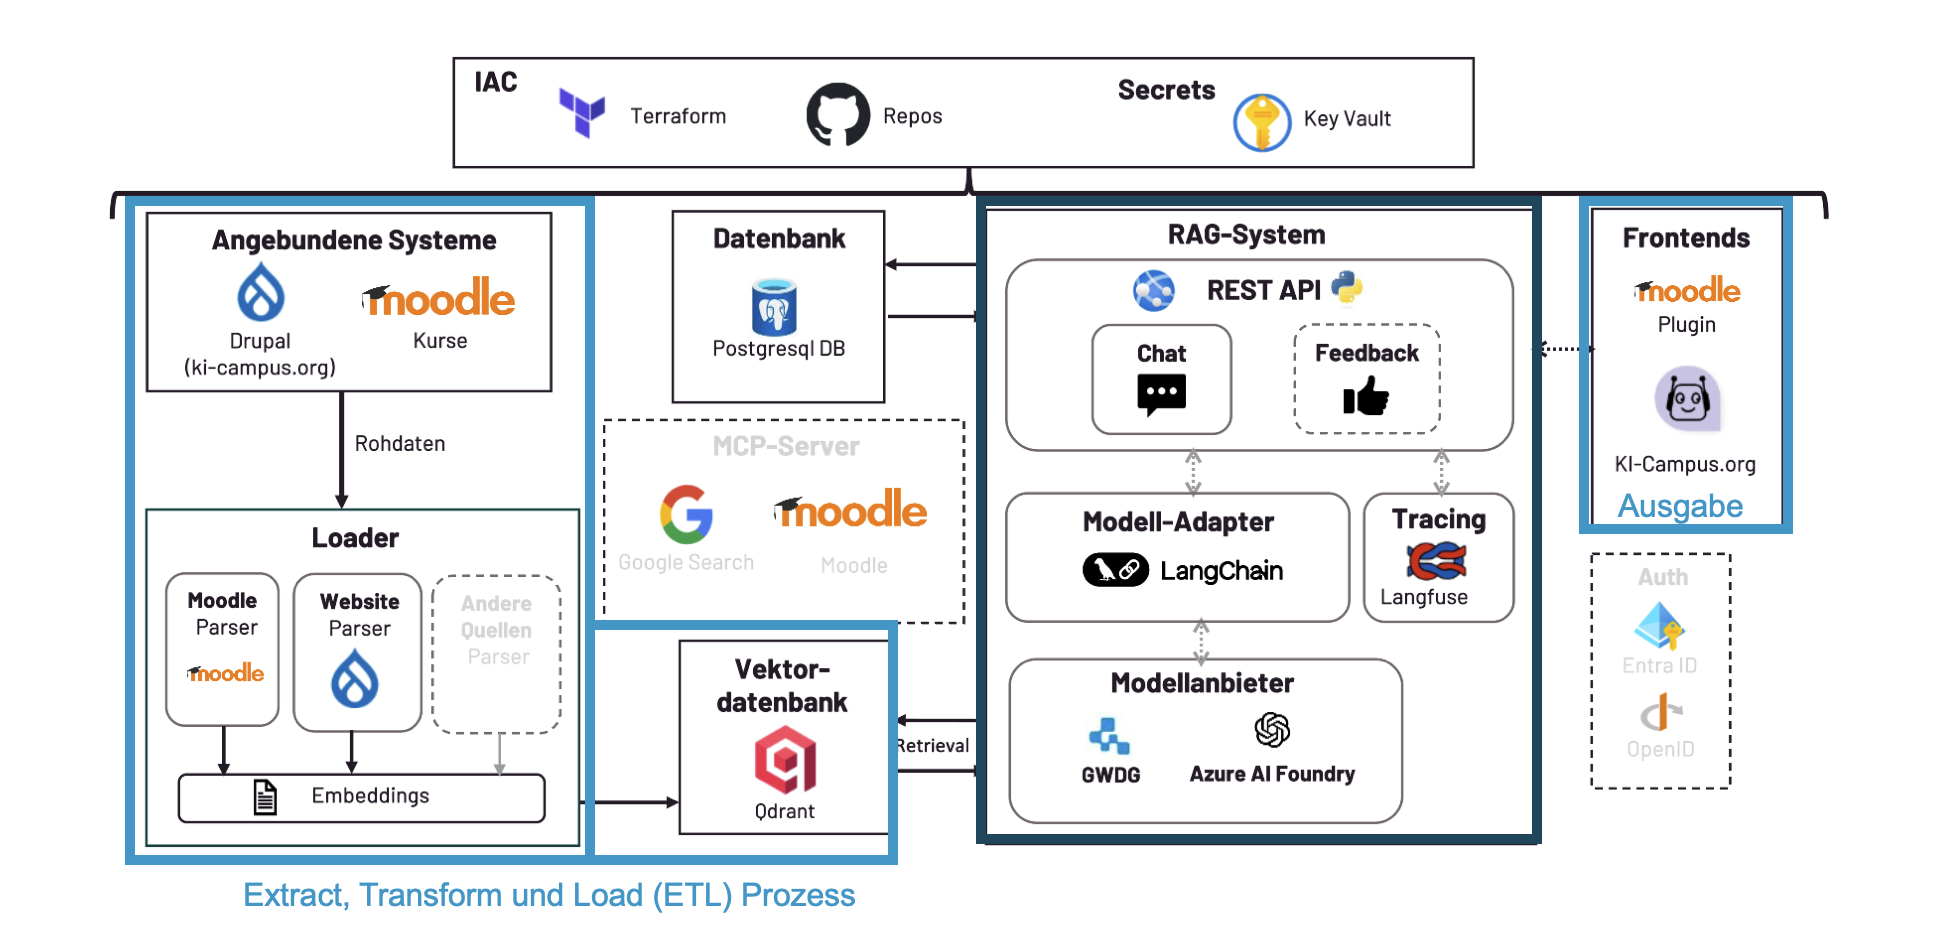
\includegraphics[width=\textwidth]{systemarchitektur_kic.png}
    \caption{Systemarchitektur des KI-Campus-Chatbots mit Datenquellen, Retrieval-System und Frontends.}
    \label{fig:kic-architektur}
\end{figure}

\section{Workflow des Retrieval-Augmented-Generation-Systems}

Der operative Ablauf des Chatbots folgt einem klar strukturierten Workflow, der die Prinzipien der Retrieval-Augmented Generation umsetzt.

Zunächst gibt ein Nutzer eine Anfrage im Frontend der Lernplattform ein. Diese Anfrage wird an das Backend-System übermittelt und dort semantisch verarbeitet. Auf Grundlage der Anfrage wird eine Vektorrepräsentation erzeugt, die mit den in der Wissensbasis gespeicherten Dokumenten verglichen wird.

Im nächsten Schritt identifiziert das Retrieval-Modul diejenigen Textsegmente, die inhaltlich am stärksten mit der Nutzeranfrage übereinstimmen. Diese relevanten Dokumentausschnitte werden anschließend dem Sprachmodell als zusätzlicher Kontext bereitgestellt.

Das Sprachmodell generiert daraufhin eine Antwort, die sowohl die ursprüngliche Nutzeranfrage als auch die abgerufenen Kontextinformationen berücksichtigt. Dadurch entsteht eine kontextualisierte und auf die KI-Campus-Inhalte bezogene Antwort.

Falls keine ausreichenden Kontextinformationen identifiziert werden können, greift das System auf vordefinierte Antwortstrategien zurück, um Fehlinformationen zu vermeiden.

Der Workflow lässt sich somit in vier Hauptschritte unterteilen:
\begin{enumerate}
    \item Nutzeranfrage
    \item semantisches Retrieval
    \item kontextbasierte Antwortgenerierung
    \item Ausgabe im Frontend
\end{enumerate}

Diese Abfolge bildet die funktionale Grundlage des Systems und dient als Ausgangspunkt für die im weiteren Verlauf des Projekts durchgeführten Optimierungen.

Abbildung~\ref{fig:kic-workflow} visualisiert die einzelnen Prozessschritte des RAG-Workflows.

\begin{figure}[H]
    \centering
    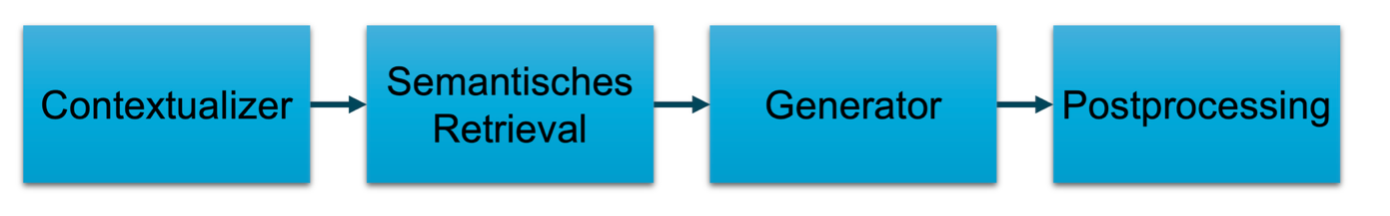
\includegraphics[width=0.95\textwidth]{workflow_kic_org.png}
    \caption{Konzeptioneller Workflow des KI-Campus-Chatbots.}
    \label{fig:kic-workflow}
\end{figure}

Trotz der modularen Architektur und des klar strukturierten Workflows zeigten sich zum Projektstart mehrere strukturelle und funktionale Limitationen. Dazu zählen eine teilweise eingeschränkte Kontextsensitivität, eine starre No-Answer-Logik sowie eine begrenzte Sprachrobustheit. Darüber hinaus zeigte sich, dass die Datenpipeline nicht alle verfügbaren Inhalte vollständig oder konsistent verarbeitete.

Diese strukturellen Eigenschaften bildeten den Ausgangspunkt für die im weiteren Verlauf des Projekts entwickelte Weiterentwicklung und Evaluation des Systems.

\chapter{Projektdesign}
\label{sec:projektdesign}

Das Projekt folgte einem strukturierten, iterativen Vorgehen, das Analyse, Entwicklung, Evaluation und Dokumentation miteinander verband. Um flexibel auf neue Erkenntnisse reagieren und kontinuierliche Verbesserungen ermöglichen zu können, wurde das Projekt entlang agiler Projektmanagementprinzipien organisiert. Die Projektstruktur gliederte sich in fünf aufeinander aufbauende Phasen:
\begin{enumerate}
    \item Onboarding
    \item Ideation \& Scoping
    \item Development
    \item Evaluation
    \item Research Documentation
\end{enumerate}
In der Onboarding-Phase erfolgten die Einarbeitung in die bestehende Systemarchitektur, das Identifizieren von Projektzielen sowie das Konkretisieren der Forschungsfrage. Zudem legten eine Marktanalyse und zwei Literaturrecherchen die wissensschaftliche Fundierung der Arbeit.

Die Phase Ideation \& Scoping diente der systematischen Identifikation von Verbesserungspotenzialen. Hierzu wurden reale Chatinteraktionen analysiert und typische Nutzungsszenarien herausgearbeitet. Auf Basis dieser Erkenntnisse wurden repräsentative Use Cases definiert, die als Grundlage für die Weiterentwicklung und Evaluation dienten. In dieser Phase wurden kreative Kollaborationstechniken wie Brainstorming und Gruppendiskussionen eingesetzt.

In der Development-Phase erfolgten strukturelle und funktionale Anpassungen des Systems, darunter Erweiterungen der Ingestion-Pipeline, Weiterentwicklung der Logik des Chatbots sowie weitere kleinere Anpassungen. Die Weiterentwicklung erfolgte iterativ in Subaufgaben (Arbeitspaketen) und wurde mittels der Plattform GitHub koordiniert.

Die Evaluation-Phase umfasste die systematische Bewertung der ursprünglichen und weiterentwickelten Systemversion. Hierfür wurde das erarbeite Evaluationskonzept umgesetzt. Abschließend wurden die Ergebnisse im Rahmen der Research Documentation konsolidiert und in Form des Projektberichts, eines Posters sowie einer Abschlusspräsentation aufbereitet.

Die operative Umsetzung der Entwicklungs- und Evaluationsschritte erfolgte auf Basis eines Kanban-Boards (siehe \autoref{anhang:b}), auf dem Arbeitspakete strukturiert und priorisiert wurden. Ein umfassendes und strukturiertes Miro-Board diente als zentrale Plattform für die Dokumentation und Visualisierung von Wissen. Regelmäßige zweiwöchentliche Meetings fungierten als Sprint Reviews, in denen Zwischenergebnisse präsentiert, technische Entscheidungen reflektiert und neue Aufgaben priorisiert wurden. Dieses Vorgehen ermöglichte eine adaptive Projektsteuerung in Reaktion auf Erkenntnisse aus Analyse- und Evaluationszyklen. Durch diese iterative Arbeitsweise konnten Entwicklungs- und Evaluationszyklen mehrfach durchlaufen und schrittweise optimiert werden. Die räumliche Nähe zu den Verantwortlichen des KI-Campus, jeden Mittwoch wurde vor Ort gearbeitet, ermöglichte eine enge Abstimmung.

Die Projektrollen waren klar verteilt: Max Landefeld (Projektleitung) verantwortete Planung, Koordination sowie das Prompt-Engineering und die Konzeption der Blindtests mit den Experten. Xhoana Garipi (Dokumentation) implementierte RAGAS, dokumentierte Ergebnisse und unterstützte Code- und Pipeline-Anpassungen. Maximilian Wilk (Research Lead) übernahm Recherche und die technische Weiterentwicklung der Logik des Chatbots. Zitho Cifire (Kommunikation) koordinierte externe Abstimmungen und entwickelte die Chatbot-Arena für das Blindtesting mit Nutzern. Veit Weber (Qualitätssicherung) verantwortete Code Reviews, Bug-Fixing sowie Optimierungen der Ingestion-Pipeline.

Inhaltlich orientierte sich das Projekt an zwei übergeordneten Zielsetzungen: Erstens der Entwicklung einer wissenschaftlich fundierten Methode zur strukturierten Bewertung von Qualitätsunterschieden in RAG-basierten Systemen. Zweitens der Ableitung und Implementierung konkret messbarer Qualitätsverbesserungen auf Basis dieser Methodik.
\input{kapitel/04_methodik}
\input{kapitel/05_ergebnisse}
\chapter{Diskussion der Ergebnisse}

\section{Einfluss der Implementierungen}
In diesem Kapitel soll diskutiert werden, welche Auswirkungen die verschiedenen Implementierungen auf die Ergebnisse der Evaluierung hatten. Die größere Vektordatenbank durch die Erweiterung der Ingestion-Pipeline sowie das hybride Retrieval und der Reranker führten zu einem starken Kontextbezug der zweiten Chatbotverseion (V2). Dies ziegt sich zum einen in der signifikant verbesserten Context Relevancy in RAGAS als auch dem Expertenblindtest, bei der sowohl der Fragebogen als auch die Kommentare eine bessere Kontextfundierung bestätigen. Die Ingestion-Pipeline macht deutlich mehr Dokumente zugänglich, sodass die Wahrscheinlichkeit steigt, dass relevante Informationen gefunden werden und dass der retrievde Kontext nicht mit UNNÖTIGEN Chunks befüllt werden muss. Das hybride Retrieval ermöglicht es, sowohl klassische Suchmethoden als auch moderne Ansätze zu nutzen, um relevante Dokumente zu identifizieren. Der Reranker verbessert die Auswahl der Dokumente, indem er die Relevanz der gefundenen Informationen bewertet und priorisiert. Damit konnte das Retrieval, wenn auch durch höhere Kosten, die zu einem späteren Zeitpunkt diskutiert werden, signifikant verbessert werden. Bei der Generation zeigt sich ein differenzierteres Bild. Die Umstellung der Logik sowie das Anpassen der Systemprompts sind hierbei die zentralen Änderungen. Dabei lassen sich die Ergebnisse gut nach Workflow unterteilen.

\begin{itemize}
    \item Haben wir Auswertung Path ohne Retrieval?
    \item Simple und Multi Hop ist zu viel
    \item Sokratischer Lernansatz gut aber nicht produktionsreif
    \item --> Diskussion über Trade-off Qualität vs. Kosten
    \item Überarbeitung der
\end{itemize}

\section{Methodenreflexion}
\label{sec:methodrefl}


\input{kapitel/07_implikationen}
\input{kapitel/08_fazit}

% -----------------------------------

\backmatter

\bibliographystyle{apacite}
\bibliography{literatur/quellen}

\appendix
\addchap{Anhang}

\addsec{Anhang A: Clustering-Skript zur thematischen Gruppierung von Chatbot-Prompts}\label{anhang:a}
\lstinputlisting[language=Python, caption={Clustering-Skript zur thematischen Gruppierung von Chatbot-Prompts (Python)}, label={lst:clustering_script}]{code/clustering_script.py}

\addsec{Anhang B: Projektplan-Timeline (Gantt-Chart)}\label{anhang:b}
\begin{landscape}
\begin{figure}[H]
    \centering
    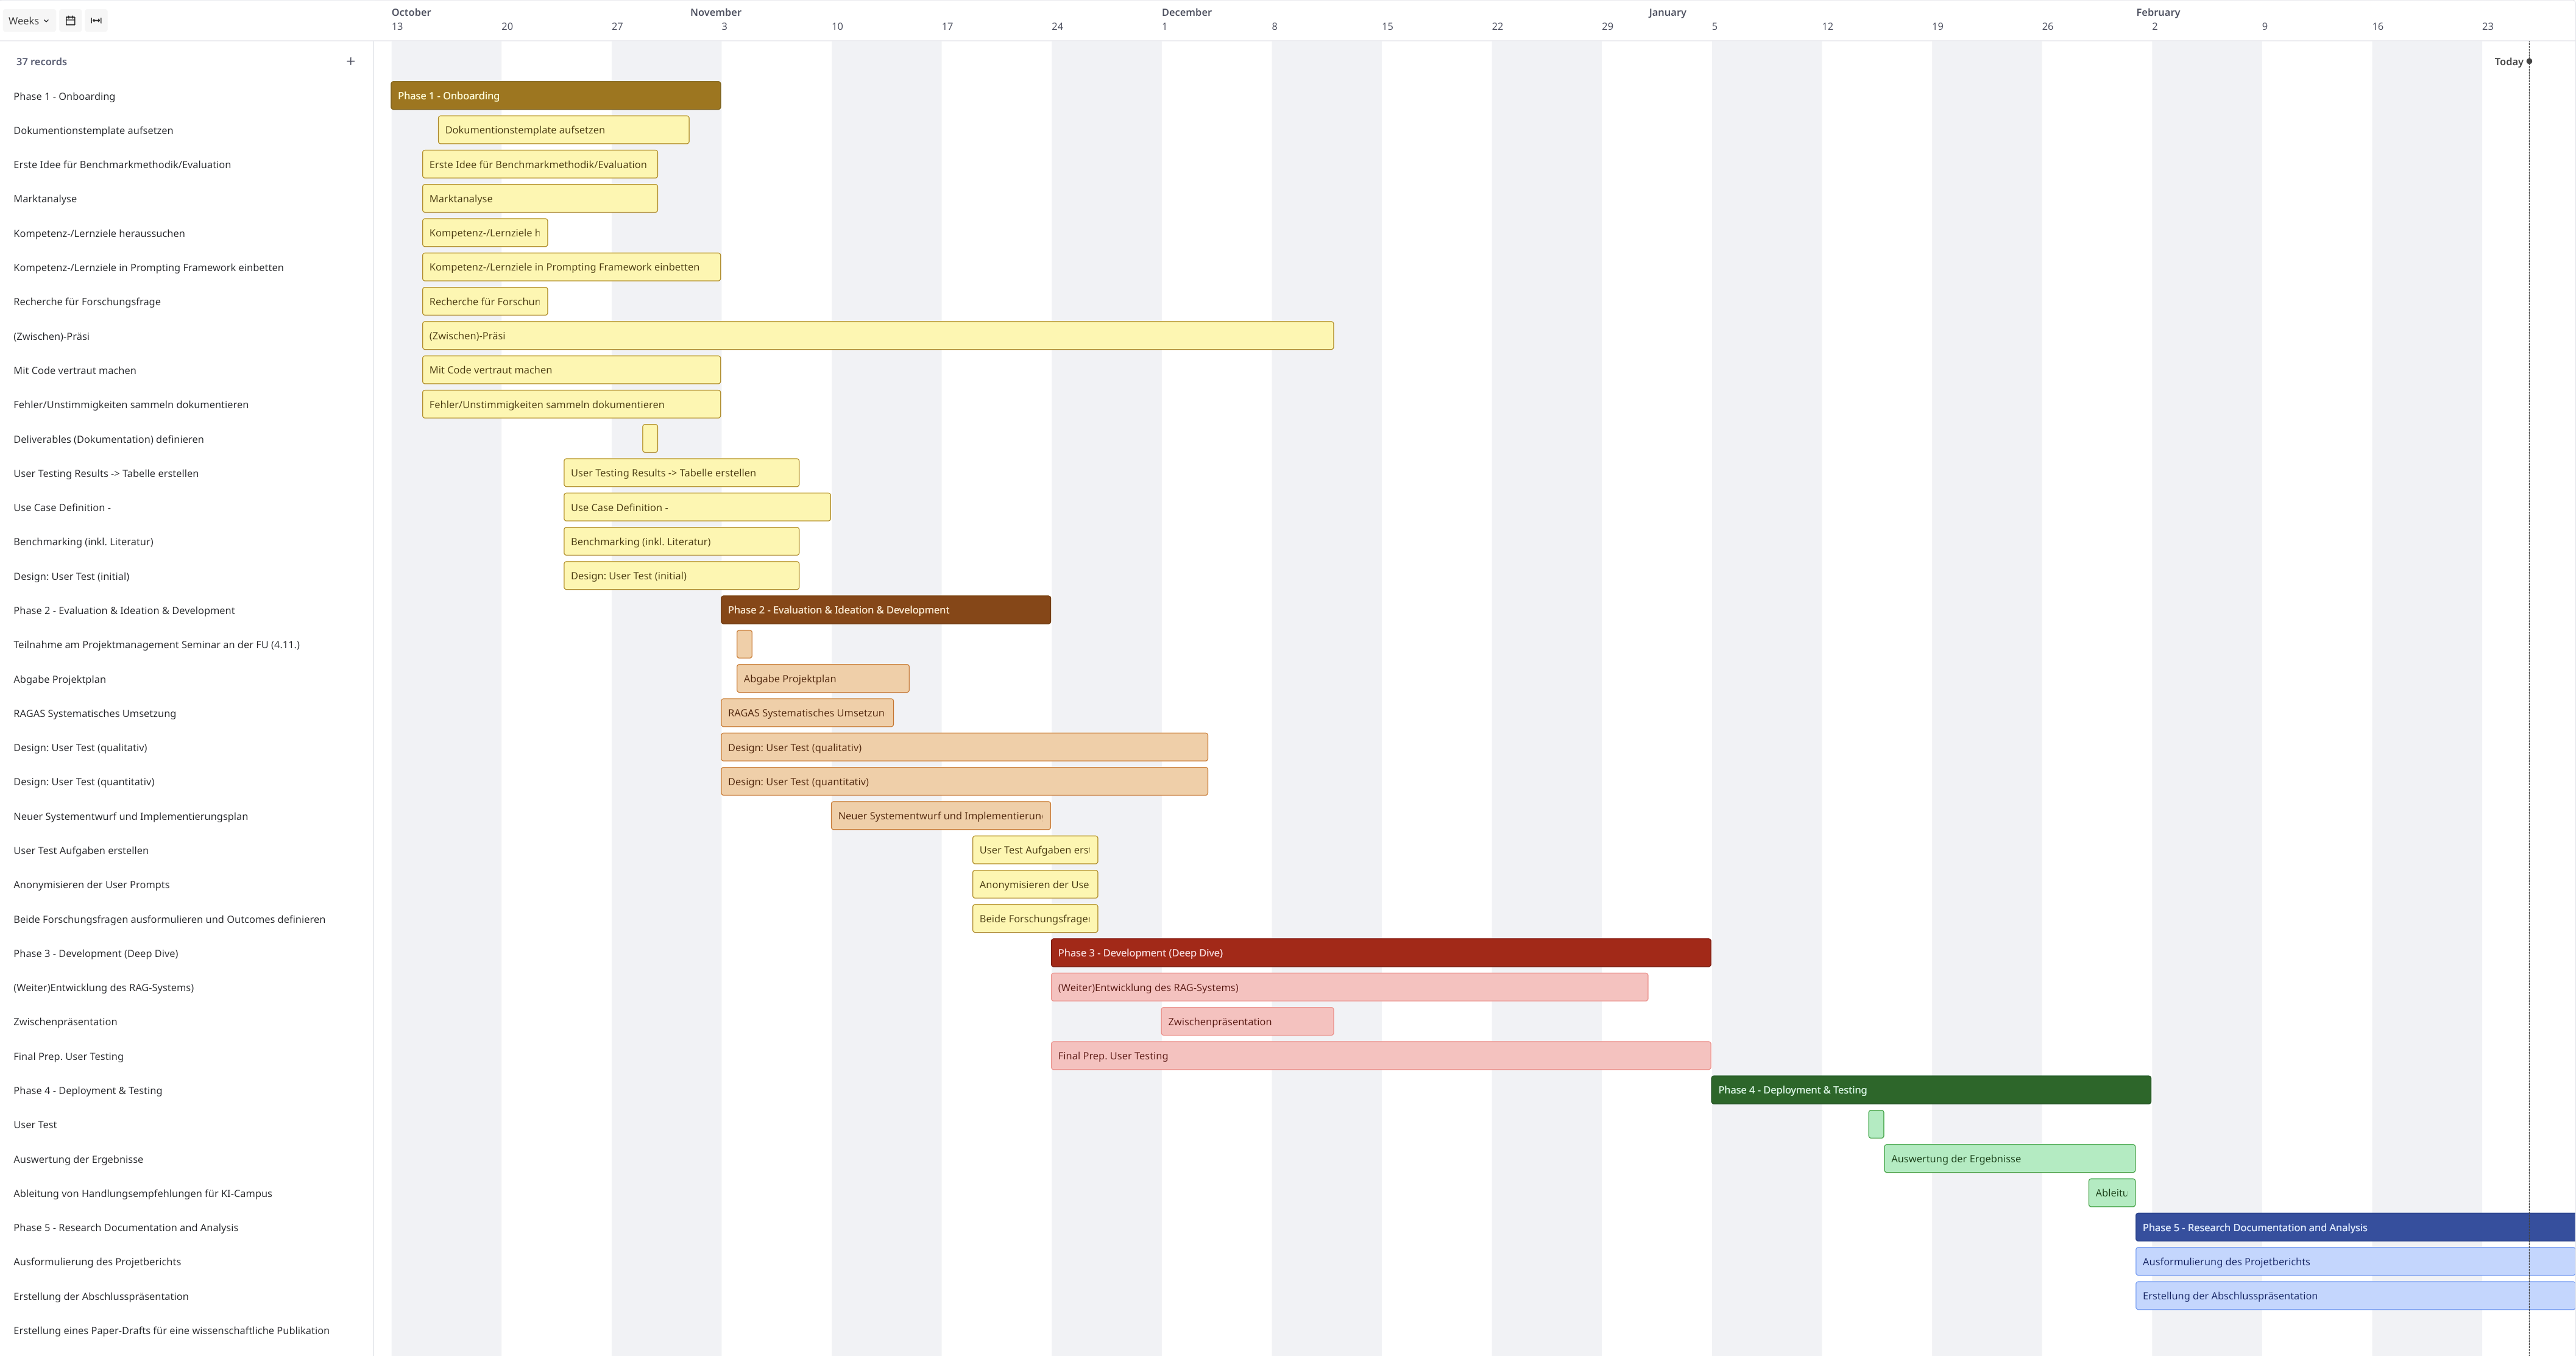
\includegraphics[width=\textwidth]{projektplan_timeline_gantt.png}
    \caption{Timeline des Projektplans als Gantt-Chart.}
    \label{fig:gantt_timeline}
\end{figure}
\end{landscape}


\input{kapitel/erklaerung}

\end{document}